\chapter{Pattern Expectation}
\label{chap:expat}
  
  %\bibentry{me-expat}

  
  In the set of all permutations of length $n$, all patterns of a fixed length 
  \emph{occur} the same number of times. However, if we restrict to smaller
  classes of permutation, the situation quickly becomes more interesting.  The
  investigation of pattern occurrences within permutations is a recent and
  productive research topic. This chapter explores this new area, and uses it
  to develop connections between permutation classes. 
  
  
  In particular, we examine the classes of $123$- and $132$-avoiding
  permutations, and show that the number of $231$ patterns is identical in each.
  This identity extends an earlier result of Mikl\'os B\'ona~\cite{Bona2012},
  and its derivation sheds further light on the distribution of pattern
  occurrences within permutation classes. Further, this chapter brings to light
  new equivalences between these classes, building on those presented by
  Elizalde~\cite{sergithesis}, and forming a foundation for
  further study~\cite{Elizalde2013, Rudolph2013, Janson2014}.  This chapter is
  based partly on~\cite{me-expat}.

  

  


% =========================================================================== %
\section{Pattern Occurrences}
\label{expat:occurrences}
  
  Our primary concern in this chapter (and much of Chapter~\ref{chap:fixpat})
  will be the number of \emph{occurrences} of a pattern within a permutation.
  The number of occurrences is the number of copies of the pattern we can
  find within a permutations; formally, we define this as follows: 
  
  \begin{definition} \label{def:occurrence} \index{pattern occurrences}
    Let $\sg = \sg_1 \sg_2 \dots \sg_k$ be a pattern of length $k$, and $\pi =
    \pi_1 \pi_2 \dots \pi_n$ a permutation of length $n$. An \emph{occurrence} of the
    pattern $\sg$ in $\pi$ is a subsequence $i_1 < i_2 < \dots < i_k$ such
    that 
    $$ \pi_{i_1} \pi_{i_2} \dots \pi_{i_k} \sim \sg_1 \sg_2 \dots \sg_k. $$ 
    The number of occurrences of $\sg$ in $\pi$, denoted by $\num_\sg(\pi)$, is
    the number of such subsequences.  
  \end{definition}
    
  For example, the permutation $\pi = 462513$ contains $2$ occurrences of the
  pattern $213$, since the first, third, and fourth, as well as the third,
  fifth, and sixth, entries of $p$ form $213$ patterns. Thus,
  $\num_{213}(462513) = 2$.  

  

  Clearly, for permutations $\pi$ of length $n$ and $\sg$ of length $k$, we have
  that $\num_q(\pi)$ is bounded below by $0$ and above by $\binom{n}{k}$. This
  minimum value is realized by taking $\pi$ to be any $\sg$-avoiding
  permutation, and the maximum is attained, for example, when both $\pi$ and
  $\sg$ are ascending permutations.  Our primary concern will be the average
  number of occurrences of a pattern over a set of permutations. In the interest
  of brevity, we will abuse the above notation to apply to sets:
  
  \begin{definition} \label{def:set-occurrence} For a given pattern $\sg$ and a
  set $S$ of permutations, let $\num_q(S)$ denote the total number of
  occurrences of $\sg$ within the set $S$. That is, $$ \num_\sg(S) = \sum_{\pi
  \in S} \num_\sg(\pi).$$ \end{definition}
  
  For example, letting $S = \{2341, 4321, 1234\}$, we have that 
  $$ \num_{123}(S) = 1 + 0 + 4 = 5.$$ 


  \subsection{Pattern Expectation}
      
    Counting the total number of occurrences of a pattern within a set of
    permutations has an alternate, probabilistic interpretation. The
    \emph{expectation} \index{expectation} of a pattern within a set is defined
    to be the average number of occurrences of the pattern within a randomly
    selected element from the set. Clearly, we have that the expectation of a
    pattern $\sg$ in a set $S$ is equal to $\num_\sg(S) / |S|$. 
    
    This probabilistic interpretation motivates many questions, several of which
    have yielded interesting and surprising answers. We start with an
    illustrative example, whose derivation showcases some of the ideas which
    will be useful later. In particular, \emph{linearity of expectation}
    \index{linearity of expectation} will prove useful. 
    
    \begin{proposition} \label{expat:prop:allperms}
      Let $\sg$ be any pattern of length $k$, and let $n \geq k$.  Then 
      $$ \num_\sg(\S_n) = \frac{n!}{k!} \binom{n}{k}.$$
    \end{proposition}
    \begin{proof}
      We show that the expectation of the pattern $\sg$ is equal to 
      $\binom{n}{k}/k!$, which will imply the desired result. 
      Let $\pi$ be a (uniformly) randomly selected permutation in $\S_n$, and let
      $X$ be the random variable denoting the number of occurrences of $\sg$
      within $\pi$. 

      There are $\binom{n}{k}$ sets of positions of $\pi$ in which a $\sg$
      pattern could possibly occur. For each set $P$, let 
      $$ X_P = \left\{ \begin{array}{cc} 
                1 & \text{ the entries of $P$ form a $\sg$ pattern} \\
                0 & \text{ otherwise} 
              \end{array}\right..
      $$

      It now follows that $X = \sum_{P} X_P$, and so by linearity of expectation,
      we have that 
      $$ \Ex{X} = \sum_P \Ex{X_P}.$$

      Finally, for any specified set of indices, all patterns are equally likely.
      Therefore, $\Ex{X_P} = 1 / k!$. Combining, we see that 
      $$ \Ex{X} = \sum_P \frac{1}{k!} = \binom{n}{k}\frac{1}{k!}. $$

      Therefore, we have that 
      $$\num_\sg(\S_n) = \frac{|\S_n|}{k!} \binom{n}{k} =
      \frac{n!}{k!} \binom{n}{k}.$$
    \end{proof}


    Fact \ref{expat:prop:allperms} shows that the total number of pattern occurrences
    within the set of all permutations depends \emph{only} on the length of the
    pattern specified. This contrasts sharply with the fact that the numbers of
    permutations which avoid a given pattern varies widely based on the choice of
    pattern. This discrepancy can be explained in part by the fact that certain
    patterns are better able to overlap with themselves, so that a smaller number
    of permutations contains a higher concentration of pattern occurrences. 
    
    The problem of pattern packing will be discussed in more detail in Chapter
    \ref{chap:fixpat}. In this chapter we examine the pattern expectation of
    of small patterns within avoidance classes. In particular we seek insight to
    the following question, first posed by Joshua Cooper: ``How does the absence
    of one pattern affect the expectation of another?''
    % TODO: cite josh cooper 


  \subsection{Background and Data}
    
    The total number of length $3$ patterns in the sets $\Av_n(123)$ and
    $\Av_n(132)$ are shown below, for $1 \leq n \leq 7$.  

    \begin{table}[t] \label{expat:tab:data}
    \caption[Total number of pattern occurrences]{Total number of pattern
        occurrences for length $3$ patterns in $123$- and $132$-avoiding
        permutations.}
    $$
    \begin{array}{ccccccc}
        \multicolumn{7}{c}{\Av_n(123) } \\
        \text{length} & \num_{123} & \num_{132} & \num_{213}
        & \num_{231} & \num_{312} & \num_{321} \\
        \hline
        3  & 0     &    1  &    1 &    1 &    1 &    1  \\
        4  & 0     &    9  &    9 &   11 &   11 &   16  \\
        5  & 0     &    57 &   57 &   81 &   81 &  144  \\
        6  & 0     &   312 &  312 &  500 &  500 & 1016  \\
        7  & 0     &  1578 & 1578 & 2794 & 2794 & 6271
      \end{array}
    $$

    \vspace{1pc}

    $$
    \begin{array}{ccccccc}
        \multicolumn{7}{c}{\Av_n(132) } \\
        \text{length} & \num_{123} & \num_{132} & \num_{213}
        & \num_{231} & \num_{312} & \num_{321} \\
        \hline
       3  & 1     &    0  &    1 &    1 &    1 &    1  \\
       4  & 10    &    0  &   11 &   11 &   11 &   13  \\
       5  & 68    &    0  &   81 &   81 &   81 &  109  \\
       6  & 392   &    0  &  500 &  500 &  500 &  748  \\
       7  & 2063  &    0  & 2794 & 2794 & 2794 & 4570
     \end{array}
    $$
    \end{table}

    Since both $123$ and $132$ are involutions, \index{involution} inversion
    maps each set to itself, and maps patterns to their inverse. This implies
    the identity $\num_{231} = \num_{312}$ in both sets of permutations.  
    Mikl\'os B\'ona~\cite{Bona2010, Bona2012} investigated the set
    $\Av_n(132)$ and enumerated the total occurrences of each length 3 pattern.
    In particular, he established the identity $\num_{213}(\Av_n(132))
    = \num_{231}(\Av_n(132))$. 

    This implies that the statistics \index{statistic} $\num_{213}$ and
    $\num_{231}$ have the same expectations \index{expectation} over the set of
    $132$-avoiding permutations of length $n$. This identity is surprising in part because
    these two statistics have \emph{different distributions} over this set, but
    share the same average value. 

    The main motivation for Section~\ref{expat:av123} is establishing the
    identity 
    $$\num_{231}(\Av(132)) = \num_{231}(\Av(123)).$$
    This identity extends B\'ona's result, and presents another example of two
    permutation statistics with different distributions having the same mean. 


    

% =========================================================================== %
\section{123-avoiding Permutations}
\label{expat:av123}

    In this section, we derive exact and asymptotic values for $\num_\sg
    (\Av_n(123))$ for $|\sg| \leq 3$ and $n \geq 0$. In addition, we show that
    for $k \geq 1$, the pattern $k\ (k-1)\ (k-2)\ \dots 2\ 1$ has a higher
    expectation than any other pattern of length $k$ for large enough permutations. 
    Finally, applying recent results of Mikl\'os B\'ona, we show that 
    the total number of $231$ patterns is identical within the sets of
    $132$-avoiding and $123$-avoiding permutations of length $n$. 


    Throughout this sections, let $n$ be some fixed positive integer. For
    simplicity of notation, we use $\num_\sg$ to denote $\num_\sg (\Av_n(123))$. 
     

  \subsection{Class Structure}

    The class of $123$-avoiding permutations has a rigid structure, which we will
    use to investigate pattern occurrences. 
    Recall (Section~\ref{prelim:sub:catalan}) that $|\Av_n(123)| = c_n$, where $c_n$
    is the $n$th Catalan number.  \index{Catalan number}.  For a permutation
    $\pi = \pi_1 \pi_2 \dots \pi_n$, we say that the entry $\pi_i$ is a
    \emph{left-to-right minimum} (ltr-min) \index{left-to-right minimum} if it
    is smaller than all of the elements to its left, and a \emph{right-to-left
    maximum} (rtl-max) \index{left-to-right maximum} if it is larger than all of
    the elements to its right. 
    
    In a $123$-avoiding permutation $\pi$, \emph{every} element is either a
    ltr-min or a rtl-max (or possibly both), since otherwise it would have a bigger
    element to its right and a smaller element to its left, which would form a
    $123$ pattern. By definition, the sets of ltr-min and of rtl-max are both
    decreasing when read from left to right. Therefore, every $123$-avoiding
    permutation is the union of two decreasing sequences of entries. 

    Breaking down permutations into these two decreasing sequences will prove
    useful in the following sections. However, the possibility of an element
    being both a ltr-min and a rtl-max poses problems. Further restricting our
    permutations will alleviate this issue. 

    \begin{definition} \label{def:indecomposable}
      A permutation $\pi = \pi_1 \pi_2 \dots p_n$ is \emph{skew-decomposable}  if
      there exist permutations $\sg$ and $\ph$ for which $\pi = \sg \ssum \ph$.
      Otherwise, we say that $\pi$ is \emph{skew-indecomposable}.  Denote the set of
      indecomposable $123$-avoiding permutation by $\Avns$. 
      Sum (in)decomposability is defined similarly. 
    \end{definition}
    
    In this chapter we consider only
    skew-(in)decomposability, and so we drop the word `skew' for the simplicity
    of notation. 


    Note that if any element of $\pi$ is both a ltr-min and a rtl-max, then $\pi$
    is decomposable. It follows then that every indecomposable 123-avoiding
    permutation can be uniquely decomposed into its left-to-right minima and its
    left-to-right maxima. Further, it follows that \emph{every} 123-avoiding
    permutation can be written as a skew sum of indecomposable 123-avoiding
    permutations. We use this fact to enumerate these permutations.


    \begin{proposition} \label{expat:prop:indecomposable}

      The number of indecomposable $123$-avoiding permutations is $c_{n-1}$, the
      $(n-1)$st Catalan number \index{Catalan number}.
    \end{proposition}
    \begin{proof}
      Let 
      $$ C^*(x) = \sum_{n \geq 0} |\Avns| x^n.$$
      We know that $|\Avn| = c_n$, and so 
      $$ \sum_{n \geq 0} |\Avn| x^n = \frac{1 - \sqrt{1-4x}}{2x} = C(x).$$
      Since every permutation $\pi \in \Avn$ can be written as $sg_1 \ssum \sg_2
      \dots \sg_k$ for some $\sg_1, \sg_2, \dots \sg_k \in \Avns$ and some $k
      \geq 1$, it follows that 
      $$ C(x) = 1 + C^*(x) + (C^*)(x))^2 + (C^*(x))^3 + \dots 
        = \frac{1}{1 - C^*(x)}.$$
      Rearranging this equation leads to 
      $$ C^*(x) = \frac{C(x) - 1}{C(x)} = xC(x).$$
      The second equality follows from the identity $C(x) = xC(x)^2 + 1$. 

      Therefore, 
      $$ \sum_{n \geq 0} |\Avns|x^n = C^*(x) = xC(x) = \sum_{n \geq 1}
      c_{n-1}x^n.$$
    \end{proof}
      

  \subsection{Patterns of Length 2}  

    To start, we compute the values $\num_{12}$ and $\num_{21}$. Since every pair
    of entries must form either a $12$ or a $21$ pattern, the sum $\num_{12} +
    \num_{21}$ is equal to the total number of pairs of entries amongst the set
    of all $123$-avoiding permutations. Therefore, we have 
    $$ \num_{12} + \num_{21} = \binom{n}{2}.$$

    An \emph{inversion} \index{inversion} of a permutation is an occurrence
    of the pattern $21$. Inversions are a well-known and well-studied
    permutation statistic, and the total number of inversions amongst the set
    $\Av_n(321)$ is known. 

    \begin{theorem}[Cheng, Eu, Fu~\cite{Cheng2007}] 
      The total number of inversions in the set $\Av_n(321)$ is given by 
      $$ \num_{21}(\Av_n(321)) = 4^{n-1} - \binom{2n - 1}{n}.$$
      The generating function for this sequence is as follows:
      $$ \sum_{n \geq 0} \num_{21}(\Av_n(321)) x^n = 
        \frac{x^2 C(x)^2}{1 - 4x}.$$
    \end{theorem}

    By reversing permutations, we see that $\num_{21}(\Av_n(321)) =
    \num_{12}(\Av_n(123))$. This allows us to establish exact answers for the
    number of occurrences of length $2$ patterns within $\Avn$. 

    \begin{proposition} \label{prop:2-patterns}
      The total number of $12$ patterns in $\Avn$ is given by 
      $$ \num_{12} = 4^{n-1} - \binom{2n - 1}{n}.$$
      Further, since 
      $ \num_{21}(\Av_n(321)) = 4^{n-1} - \binom{2n - 1}{n},$
      it follows that 
      $$ \num_{21} = \binom{n}{2} c_n - 4^{n-1} + \binom{2n - 1}{n}.$$
    \end{proposition}


  \subsection{Patterns of Length 3}

    Deriving the number of occurrences for length three patterns is considerably
    more involved, but utilizes some of the same ideas. In this section we find
    both the asymptotic and exact values for the total occurrences of $\num_\sg$
    for each $\sg \in \S_3$.  The key idea will be derive the total number of
    occurrences of a single pattern, and then use the class structures to develop
    the other values. 
    Let 
    $$a_n = \num_{213}, \quad b_n = \num_{231}, \quad \num_{321}.$$



    We start by finding the generating function for the numbers
    $\num_{213}(\Avns)$. While this may seem arbitrary, this will in fact lead
    to generating functions for all other patterns.  Let $\pi$ be a permutation
    in $\Avns$. Recall that each entry in $\pi$ is either a ltr-min or a
    rtl-max, and no entry is both. An occurrence of $213$ within $\pi$ must
    consist of two left-to-right minima followed by a right-to-left maximum. By
    counting the number of entries to the left and below each rtl-max we can
    exactly determine the number of $213$ patterns within $\pi$. 
    
    \begin{lemma} \label{lemma:213pats}
      The generating function $A^*(x)$ for the number of $213$ patterns in
      $\Avns$ is given by
      $$ A^*(x) = \sum_{n\geq 0} \num_{213}(\Avns) =
      \frac{x^3C(x)}{(1-4x)^{3/2}} = \frac{x^2}{2(1-4x)^{3/2}} -
      \frac{x^2}{2(1-4x)}.$$
    \end{lemma}
    \begin{proof}
      The proof consists of three parts: First, we examine the structure of
      permutations in $\Avns$, and find a simple way of counting the number of
      $213$ patterns. Second, we build a bijection onto Dyck paths which maps
      $213$ patterns to a path statistic. Finally, we find the weighted sum of
      all Dyck paths with respect to this statistic.

      The idea of the proof is as follows: We build a bijection from the set of
      permutations $\Avns$ to the set $\D$ of elevated Dyck paths of semilength
      $n$, find a statistic on these paths which corresponds to $213$ patterns,
      and then find the weighted sum of all Dyck paths with respect to this
      statistic.

      Let $\pi$ be a permutation in $\Avns$, and consider the plot of $\pi$.
      Note that, by the indecomposability of $\pi$, there is no entry which is
      simultaneously a ltr-min and a rtl-max. Construct a Dyck path $\phi(\pi)$
      of semilength $n-1$ as follows. First, build a path from $(1,n)$ to
      $(n,1)$ using the steps $\{\vect{1,0}, \vect{0,1} \}$. Let this path be
      the be the unique path which minimizes the area underneath itself while
      lying above all of the entries of $\pi$. This path, a variation of the
      construction presented in Section~\ref{prelim:sec:av123}, is then
      uniquely defined by the locations of the right-to-left maxima, which in
      turn uniquely define the permutation. Finally, rotate each $\vect{1,0}$
      step to be an up step, and each $\vect{0,-1}$ to become a downstep in
      the path $\phi(\pi)$. See Figure~\ref{expat:fig:dyckproof} for an example
      construction. 
      
      This path is a slight modification of the path given by Krattenthaler's
      bijection~\cite{Krattenthaler2001}, taking advantage of the
      indecomposability of the permutation to yield a more geometric description.
      This geometric interpretation of the bijection gives some additional
      insight into the number of $213$ patterns. 



    \begin{figure}[t] \centering
      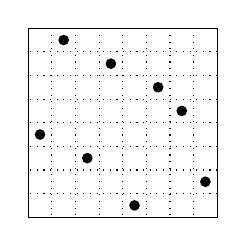
\begin{tikzpicture}[scale=.3, yscale=-1, xscale=-1]
        \draw (1,1) -- (1,9) -- (9,9) -- (9,1) -- cycle;
        \foreach \y [count = \x] in {7,4,3,8,2,6,1,5}{
          \draw[fill = black] (\x+.5,\y+.5) circle (2mm);
        }
        \foreach \i in {1, ...,9}{
          \draw[dotted] (\i,1) -- (\i,9);
          \draw[dotted] (1,\i) -- (9,\i);
        }
      \end{tikzpicture}
      \hspace{2pc}
      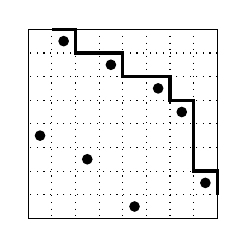
\begin{tikzpicture}[scale=.3, yscale=-1, xscale=-1]
        \draw (1,1) -- (1,9) -- (9,9) -- (9,1) -- cycle;
        \foreach \y [count = \x] in {7,4,3,8,2,6,1,5}{
          \draw[fill = black] (\x+.5,\y+.5) circle (2mm);
        }
        \foreach \i in {1, ...,9}{
          \draw[dotted] (\i,1) -- (\i,9);
          \draw[dotted] (1,\i) -- (9,\i);
        }
        \draw[very thick] (1,8) --++ (0,-1) --++ (1,0) --++ (0,-3)
                          --++ (1,0) --++(0,-1) --++(2,0) 
                          --++ (0,-1) --++ (2,0) --++(0,-1) 
                          --++ (1,0);
      \end{tikzpicture}
      \hspace{2pc}
      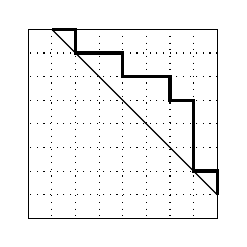
\begin{tikzpicture}[scale=.3, yscale=-1, xscale=-1]
        \draw (1,1) -- (1,9) -- (9,9) -- (9,1) -- cycle;
        \foreach \i in {1, ...,9}{
          \draw[dotted] (\i,1) -- (\i,9);
          \draw[dotted] (1,\i) -- (9,\i);
        }
        \draw (1,8) -- (8,1);
        \draw[very thick] (1,8) --++ (0,-1) --++ (1,0) --++ (0,-3)
                          --++ (1,0) --++(0,-1) --++(2,0) 
                          --++ (0,-1) --++ (2,0) --++(0,-1) 
                          --++ (1,0);
      \end{tikzpicture}
      \hspace{2pc}
      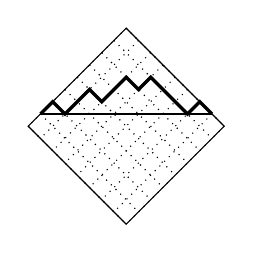
\begin{tikzpicture}[scale=.22, xscale=-1]
      \begin{scope}[shift={(3,5)},rotate=-45, yscale=-1]
        \draw (1,1) -- (1,9) -- (9,9) -- (9,1) -- cycle;
        \foreach \i in {1, ...,9}{
          \draw[dotted] (\i,1) -- (\i,9);
          \draw[dotted] (1,\i) -- (9,\i);
        }
        \draw (1,8) -- (8,1);
        \draw[very thick] (1,8) --++ (0,-1) --++ (1,0) --++ (0,-3)
                          --++ (1,0) --++(0,-1) --++(2,0) 
                          --++ (0,-1) --++ (2,0) --++(0,-1) 
                          --++ (1,0);
        \end{scope}
        \end{tikzpicture}
    \caption{The construction of the Dyck path $\phi(48371652) =
                uduuduududddud$. }
    \label{expat:fig:dyckproof}
    \end{figure}




      Note that each rtl-max in $\pi$ produces a peak in $P$. If $\pi_i$ is a
      rtl-max, let the \emph{span of $\pi_i$} ($\Sp \pi_i$) denote the number
      of entries to the left and below this entry. It follows then that 
      $\pi_i$ corresponds to a peak of height $\Sp \pi_i$ above the $x$-axis in $P$.
      An occurrence of $213$ must have a rtl-max as its $3$ entry, and it
      follows then that the $21$ entries must lie in the span of this entry. We
      therefore see that every rtl-max is involved in $\binom{\Sp \pi_i}{2}$
      occurrences of $213$, since we need only choose any two elements in its
      span to act as the $21$. 
      Therefore, if we let $h_{n,k}$ denote the total number of peaks of height
      $k$ in all Dyck paths of semilength $n$, we have that
      $$ \num_{213}(\Avns) =\sum_{k = 1}^{n-1} \binom{k}{2} h_{n-1,k}.$$

      Finally, we can compute $H(x,u) = \sum_{n,k \geq 0} h_{n,k} x^n u^k$ as
      follows. First, note that since each Dyck path begins with an upstep it has
      a unique first point at which the path returns to the $x$-axis, so we can
      decompose each path $P$ of length $n$ into the concatenation of two shorter
      paths $Q$ and $R$. This gives that $P = uQdR$, where $u$ denotes an upstep
      and $d$ a downstep, and each peak of height $k-1$ in $Q$ and height $k$ in
      $R$ leads to a peak of height $k$ in $P$. With this in mind, we have the
      following generating function relation: $$ H(x,u) = ux(H(x,u)+1)C(x) +
      xH(x,u)C(x) .$$ Here the first term counts the peaks from the $uQd$ part,
      including the case when $Q$ is empty. The second term counts the
      contribution from the $R$ part.  Rearranging leads to 
      $$ H(x,u) = \frac{uxC(x)}{1-uxC(x)-xC(x)}.$$

      Now, to count $213$ patterns, we need to count each peak with weight
      $\binom{k}{2}$. By taking derivatives twice with respect to $u$, setting
      $u=1$, dividing by two and scaling by $x$, we find that
      $$ \begin{aligned}
      \sum_{n,k \geq 0} \binom{k}{2} h_{n-1,k}x^n &
      = x \frac{\left. \partial_u ^2 H(x,u)\right|_{u=1}}{2}
      = \frac{x^3C(x)}{(1-4x)^{3/2}} \\
      & = x^3 + 7x^4 + 38x^5 + 187x^6 + 874x^7 + \dots \ .
      \end{aligned}
      $$

      The sequence $0,0,1,7,38,187\dots$ is \OEIS{A000531}.  Finally,
      the correspondence between peaks and $213$ patterns completes the proof.
    \end{proof}


  
    Now, it is relatively simple to move from the set of indecomposable
    $123$-avoiding permutations to the larger set of all $123$-avoiding
    permutations.

    \begin{theorem} \label{expat:thm:213pats}
      Let $a_n$ be the number of $213$ patterns in $\Av_n 123$. Then
      $$ \sum_{n\geq 0} a_n x^n = \frac{x^3C(x)^3}{(1-4x)^{3/2}} =
          \frac{x-1}{2(1-4x)} - \frac{3x-1}{2(1-4x)^{3/2}}.$$
    \end{theorem}
    \begin{proof}
      Let $A(x)$ be the generating function for the numbers $a_n$, and let
      $A^*(x)$ denote the generating function for the number of $213$ patterns
      in \emph{indecomposable} $123$-avoiding permutations.

      Now, any permutation $\pi$ in $\Av(123)$ can be written uniquely as a
      skew sum of a nonempty indecomposable $123$-avoiding permutation $\sg$
      and another, possibly empty, $123$-avoiding permutation $\ph$. Now, it is
      clear that any $213$ pattern in $\pi$ must be contained entirely in
      either $\sg$ or $\ph$. This leads to the following relation:
      $$ A(x) = A^*(x)C(x) + xC(x)A(x).$$
      Solving for $A$ gives
      $$ A(x) = \frac{A^*(x) C(x)}{1-xC(x)} = C^2(x) A^*(x).$$
      Lemma~\ref{lemma:213pats} now implies
      $$ A(x) = \frac{x^3 C(x)^3}{(1-4x)^{3/2}}.$$
      % Exact formula for the numbers $a_n$ is obtained from the
      % generating function by expanding by partial fractions.
    \end{proof}


    From here, we obtain the generating functions of the other patterns simply
    by relating their enumerations with the one already obtained. The following
    two observations provide linear relations between these numbers. The first
    follows from the simple fact that any three entries must form \emph{some}
    $3$-pattern. 

    \begin{lemma} \label{expat:lem:totalpats}
      On the set $\Avn$, we have that 
      $$ \num_{132} + \num_{213} + \num_{231} + \num_{312} + \num_{321} 
        =  c_n \binom{n}{3}. $$
    \end{lemma}
    \begin{proof}
      Both sides count the total number of $3$-patterns within the class
      $\Avn$.  The right-hand-side is the total number of ways of choosing
      three indices in any $123$-avoiding permutation. Each of these choices 
      is an occurrence of a $3$-patterns other than $123$, which is counted by
      the left-hand-side. 
    \end{proof}

    The next lemma provides a relationship between the numbers $\num_{132},
    \num_{213}, \num_{231}$, and $\num_{312}$ by counting the total number of
    $3$-patterns which contain a \emph{non-inversion} (an occurrence of $12$).

    \begin{lemma} \label{expat:lem:twopats}
      The following equality holds on the set $\Avn$: 
      $$ 2 \num_{132} + 2 \num_{213} + \num_{231} + \num_{312} = 
        (n-2) \num_{12} .$$
    \end{lemma}
    \begin{proof}
      Rewrite this equation as 
      $$ 
      (n-2) \num_{12} - (\num_{132} + \num_{213})
      = \num_{132} + \num_{213} + \num_{231} + \num_{312}.
      $$
      Both sides count the total number of length 3 patterns which contain at
      least one non-inversion. Indeed, the right-hand-side
      counts all 3-patterns except for $321$. The left-hand-side builds such a
      pattern by first choosing a $12$ pattern, and then adding another entry
      to create a 3-pattern. However, this overcounts the patterns $132$ and
      $213$, since each of these contains two $12$-patterns, so we subtract
      these off to correct the equality. 
    \end{proof}

    The generating functions for the numbers $c_n \binom{n}{3}$ and $(n-2)
    \num_{12}$ can be determined from the generating functions we already have.
    These equations can be obtained using techniques explained in Section
    \ref{prelim:sec:ascents-example}. 

    \begin{lemma} \label{expat:lem:genfcns}
      Letting $J(x) = \sum_{n \geq 0} \num_{12}(\Avn) x^n$, the following
      identities hold:
      $$ \begin{aligned}
      \sum_{n \geq 0} c_n \binom{n}{3} 
      &= \frac{x^3 \ddxc (C(x))}{6} \\ 
      \sum_{n \geq 0} (n-2)\num_{12}(\Avn) 
      &= x^3 \ddx \left(\frac{J(x)}{x^2} \right). 
      \end{aligned} $$
    \end{lemma}

      

    Lemmas~\ref{expat:lem:twopats} and ~\ref{expat:lem:totalpats}, coupled with
    Lemma~\ref{expat:lem:genfcns}, establish a system of linear equations with
    three unknowns, $\num_{213}, \num_{231}$, and $\num_{321}$.
    Any new linear relation or solution to one of these would solve the system,
    giving generating functions and exact formulas for the number of all length
    $3$ patterns within $\Av_n(123)$. 

    The calculation of the $\num_{213}$ provides that missing piece, but we
    note that there are many other identities which, once these lemmas are
    established, are equivalent to Theorem~\ref{expat:thm:213pats}. We collect
    some of these in Corollary~\ref{expat:cor:equivalences}. A direct proof of
    any of them could help to simplify the arguments presented here while
    retaining all of the same results, and provide further insight into the
    connections between $\Av(123)$ and $\Av(132)$. While each of these
    seem tractable to bijective methods, they have resisted many attempts at a
    direct proof  and we include them here partly out of spite.
    First, we present the generating functions for the occurrences of $231$ and
    $321$, which follow by routine (but technical) computation. 
    
    

    \begin{theorem} \label{expat:thm:231pats}
      The number of $231$ (or $312$) occurrences is given by 
      $$\sum_{n \geq 0} \num_{231}(\Av_n(123)) z^n=
      \frac{3z-1}{(1-4z)^{2}} - \frac{4z^2 - 5z + 1}{(1-4z)^{5/2}}.$$
    \end{theorem}

    \begin{corollary} \label{expat:cor:bridge}
      The total number of $231$ occurrences in $\Av_n(123)$ is equal to the
      number in $\Av_n(132)$. 
    \end{corollary}

    \begin{theorem}
      The number of $321$ occurrences is given by 
      $$
        \sum_{n\geq 0} \num_{321}(\Av_n (123)) z^n =
        \frac{ 8z^3 - 20z^2 + 8z - 1}{(1-4z)^{2}}
        - \frac{36z^3 - 34z^2 + 10z - 1}{(1-4z)^{5/2}}.
      $$
    \end{theorem}


    \begin{corollary} \label{expat:cor:equivalences}
      The following identities hold 
      $$ \num_{21}(\Avn) = 2\num_{213}(\Avns) $$
      $$ \num_{213}(\Avn) + \num_{231}(\Avn) = \num_{231} (\Av
      _{n-1}^*(123))$$
      $$ C(z) \left(\sum_{n\geq 0} \num_{213}(\Avn) z^n \right) =
        z C'(z) \left(\sum_{n \geq 0} \num_{12}(\Avn)z^n \right) $$
      $$ \sum_{n\geq 0} \num_{213} (\Av_n^* (132)  z^n) =
        \sum_{n \geq 0} \big(\num_{132}(\Avns) +
        \num_{231}(\Avns)\big)z^n. $$
    \end{corollary}




  Now we can do some analysis of the main sequences. Using some
  standard generating function analysis \cite{flajolet}, we find
  that the asymptotic growth of the number of length $3$ patterns are
  as follows:

  \vspace{1pc}

  $$ \begin{aligned}
   \num_{213} (\Avn) &\sim \sqrt{\frac{n}{\pi}} 4^{n-1} \\
   \num_{231} (\Avn) &\sim \frac{n}{2} 4^{n-1}  \\
   \num_{321} (\Avn) &\sim \frac{2}{3} \sqrt{\frac{n^3}{\pi}} 4^{n-1}. 
  \end{aligned} $$

  We see that the three sequences each differ by a factor of
  approximately $\sqrt{n}$. Surprisingly, this is the same factor that
  the sequences $\num_{123}, \num_{231}, \num_{321}$ differ by in the
  class $\Av (132)$, as seen in \cite{Bona2012}.

  Each of these generating functions are simple enough that exact
  formulas can be obtained with relatively little hassle. One could
  argue that the asymptotic values are more interesting and
  provide more insight than the complicated formulas, but we present
  them here for completeness.

  \begin{corollary}
    Let $a_n = \num_{132}(\Avn)$, $b_n = \num_{213}(\Avn)$, and $d_n =
    \num_{321}(\Avn)$. Then we have that
    $$ a_n = \frac{n+2}{4} \binom{2n}{n} - 3 \cdot 2^{2n-3} $$

    \vspace{1pc}

    $$ b_n = (2n-1) \binom{2n-3}{n-2} - (2n+1)\binom{2n-1}{n-1} +
       (n+4) \cdot 2^{2n-3}$$
    
    \vspace{1pc}

    $$ \begin{aligned} d_n
        = \frac{1}{6} \binom{2n+5}{n+1} \binom{n+4}{2}
        &- \frac{5}{3} \binom{2n+3}{n} \binom{n+3}{2}
        + \frac{17}{3} \binom{2n+1}{n-1} \binom{n+2}{2} \\
        &- 6\binom{2n-1}{n-2} \binom{n+1}{2} - (n+1) \cdot 4^{n-1}.
      \end{aligned}
    $$
  \end{corollary}

 


%===================================================================%
\subsection{Larger Patterns}

  Some of these same techniques are applicable to larger patterns.  For
  example, we can easily modify Lemmas~\ref{expat:lem:twopats}
  and~\ref{expat:lem:totalpats} to apply to patterns of all sizes. This leads to
  increasingly complicated expressions, but this simple idea can be used to
  prove the following proposition. 

  \begin{proposition}
    Let $k \in \mathbb{Z}^+$, and $\sg$ be any permutation in $\S_k$
    other than the decreasing permutation. Then for $n$ large enough,
    we have that
    $$\num_{k \dots 3 2 1}(\Avn) > \num_{\sg}(\Avn).$$
  \end{proposition}

  \begin{proof}
    Let $\cD$ be the set of permutation in $\S_k$ which are not the
    decreasing permutation.  As in Lemma~\ref{expat:lem:twopats},  we can
    express the number $\binom{n-2}{k-2}\num_{12}(\Avn)$ as a positive linear
    combination of all of $\num_{\sg} (\Avn)$ where $\sg \in \cD$. As in
    Lemma~\ref{expat:lem:totalpats}, we can express $\binom{n}{k} c_n$ as the sum
    of all $\num_{\ro} (\Avn)$ where $\ro \in \S_n$.  It follows that there is
    a positive integer $m$ and positive
    integers $e_i$ such that
    $$ \binom{n}{k} c_n - m\binom{n-2}{k-2} \num_{12} (\Avn) = \num_{k \dots
    321} - \sum_{\sg \in \cD} e_i \num_{\sg} (\Avn).$$ Asymptotic analysis
    shows that the left hand side is eventually positive, and so the first term
    on the right side eventually outgrows the second term, which completes the
    proof.
  \end{proof}



  






